\documentclass[compsoc]{IEEEtran}
\usepackage{graphicx}
\usepackage{amsmath}
\usepackage{authblk}
\usepackage[english]{babel}
\usepackage{blindtext}
\usepackage[ruled,vlined,linesnumbered]{algorithm2e}
\usepackage{algorithmic,float}
\usepackage{setspace}
\usepackage{amsfonts}
\usepackage{hyperref}
\graphicspath{ {./images/} }
\usepackage{subfig}
\usepackage{fontspec}
\usepackage{listings}
\usepackage{amsmath}
\usepackage{mathabx}
\usepackage[bottom]{footmisc}
\newfontfamily\listingsfont[Scale=.7]{inconsolata}\usepackage[font=footnotesize,labelfont=bf]{caption}
\captionsetup[algorithm2e]{font=footnotesize}
\usepackage[table,xcdraw]{xcolor}
\usepackage[utf8]{inputenc}
\title{Assignment: Checkerboard classification problem}
\author{David Bertoldi -- 735213 \\ email: d.bertoldi@campus.unimib.it}
\affil{Department of Informatics, Systems and Communication}
\affil{University of Milano-Bicocca}
\date{October 2022}

\definecolor{mGreen}{rgb}{0,0.6,0}
\definecolor{mGray}{rgb}{0.5,0.5,0.5}
\definecolor{mPurple}{rgb}{0.58,0,0.82}
\definecolor{backgroundColour}{rgb}{0.95,0.95,0.92}

\lstdefinestyle{CStyle}{
    backgroundcolor=\color{backgroundColour},   
    commentstyle=\color{mGreen},
    keywordstyle=\color{magenta},
    keywordstyle=[2]{\color{lime}},
    morekeywords=[2]{;},
    numberstyle=\tiny\color{mGray},
    stringstyle=\color{mPurple},
    basicstyle=\linespread{1}\listingsfont,
    breakatwhitespace=false,         
    breaklines=true,                 
    captionpos=b,                    
    keepspaces=true,                 
    numbers=none,                    
    numbersep=5pt,                  
    showspaces=false,                
    showstringspaces=false,
    showtabs=false,                  
    tabsize=2,
    language=C++
}

\begin{document}

\maketitle 



\section{Inspecting the data}
The data provided consists of an set of points $X \in \{(x_1, x_2) | 10 \leq x_1, x_2 \leq 20\}$ and a set of binary labels $y \in \{0, 1\}$.
The points in $X$ follow a uniform distribution with mean $\mu = 14.97$ and variance $\sigma = 8.3$; the $0$s and $1$s in $y$ are quite uniformely distributed with 
a mean of $\mu = 0.498$. \par
If we map each point $i \in X$ with the $i^{th}$ element of $y$ and assign for each element of $y$ a different color we get a \emph{check pattern} over the points of $X$, partitioning the 4000 points in 6 columns and 6 rows.
The result can be observed in Figure \ref{fig:checkerboard}

\begin{figure}[ht!]
\centering                                                                        
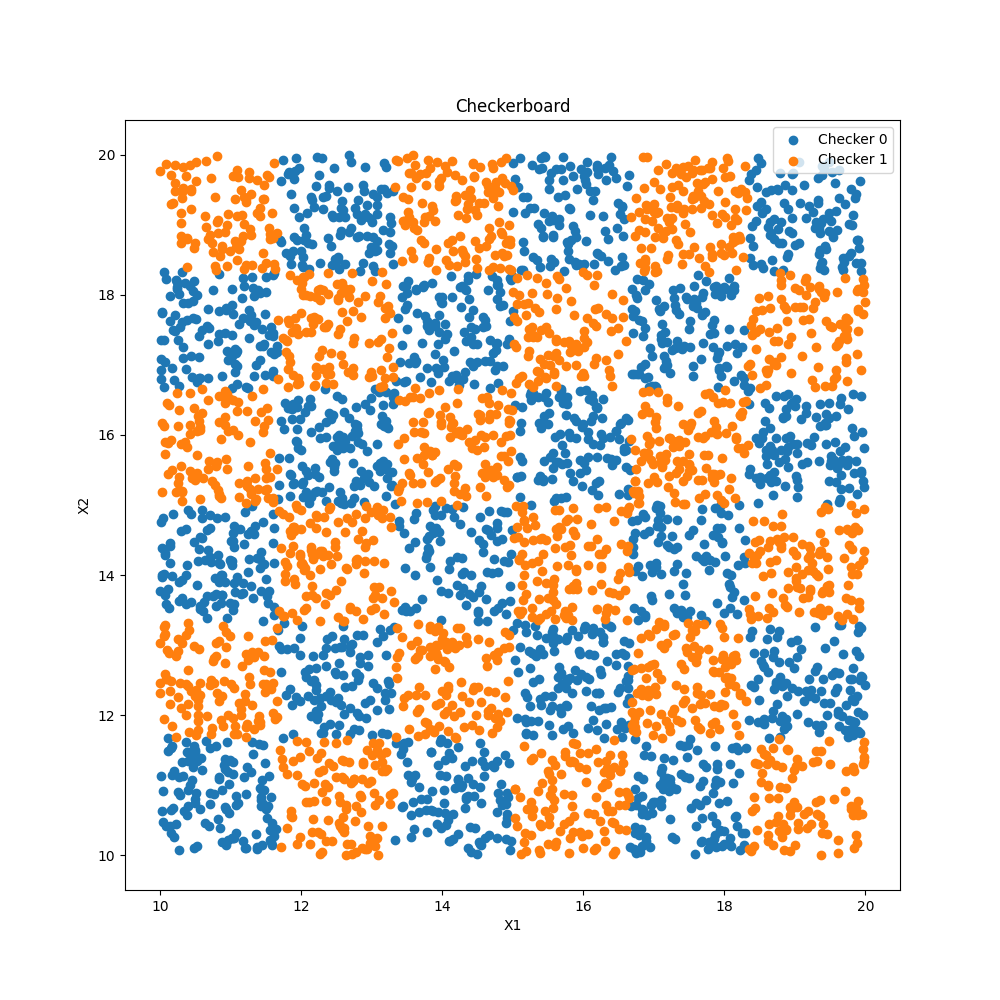
\includegraphics[width=3.5in]{../images/checkerboard.png}
\captionsetup{justification=centering}                                                                                                                                   
\caption{Visualization of the dataset}
\label{fig:checkerboard}                                                                                                                                                           
\end{figure}

\section{Preparing the data}
Before using the data we want to standardize features by removing the mean and scaling to unit variance. Standardization of a dataset is a common requirement for many machine learning estimators: they might behave badly if the individual features are not standard normally distributed. That's why we want to remove the mean $\mu$ and scale $\sigma$ to unit variance. \par
In order to do so, we use the \texttt{StandardScaler} from \texttt{sklearn.preprocessing} package. After this operation we have  $\mu=1.4 \cdot 10^{-9}$ (very close to 0) and $\sigma = 1$, which is exactly what we wanted.

\section{Building the network and training}
\subsection{Data split}
The dataset does not provide a set of points to be used for validation and testing. So we split the dataset into three partitions: 72\% of points are used for the training, 18\% for validation and 10\% for testing. Having less points used for training had proved to perform worse.

\subsection{Network}
The network chosen is a Feed-Forward Neural Network with non-linear activation functions. We tried two approaches: \texttt{tanh} and \texttt{LeakyReLU}. The first one seemed to be right choice because it is possible to emulate the check pattern with the following formula:
\[sin(y) \leq cos(x)\]
and since the definition of $tanh(x)$ can be derived from $cos(ix)$ and $sin(ix)$, there could had been some facilitation on using such activator. Unfortunately, despite the good results,
\texttt{LeakyReLU} performed better and for this reason we used it as a definitive one. \par

Because we are trying to classify points between two classes, the output function is a sigmoid. \par

Finally, the network architecture is composed by 4 hidden dense layers of rispectively 200, 150, 100 and 50 nodes. We tried with less hidden layers (2 and 3) and less nodes for each
layer (100, 50, 25, 10) but the performance where worse in terms of convergence speed and decision boundaries. Since the different configurations have similar training times, we chose this configuration over a lighter one.

Each node uses \texttt{LeakyReLU} as activator function with $\alpha=0.1$. The output node computes the sigmoid logistic function so that the output ranges between $0$ and $1$.

\begin{figure}[ht!]
\centering                                                                        
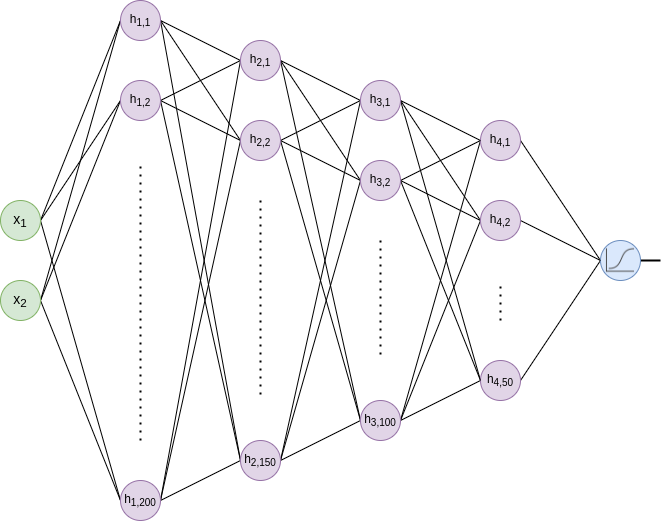
\includegraphics[width=3.5in]{../images/nn-1.png}
\captionsetup{justification=centering}                                                                                                                                   
\caption{The neural network with 4 dense hidden layers}
\label{fig:nn}                                                                                                                                                           
\end{figure}

\subsection{Training}
The choice of the optimizer was among \emph{SGD}, \emph{RMSProp} and \emph{Adam}. We tried all of them and chose \emph{Adam} 
with learning rate of $0.001$, $\beta_{1}=0.9$ and $\beta_{2}=0.999$ because it seemed to escape better from local minima, converging faster and giving better accuracy. \par
Because we are treating a binary classification problem, we used the \emph{binary crossentropy} loss function.
Figure \ref{fig:decision} shows how the decision boundaries evolve over the test dataset every 10 epochs.

\begin{figure}[ht!]
\begin{tabular}{cccc}
\subfloat[1 epoch]{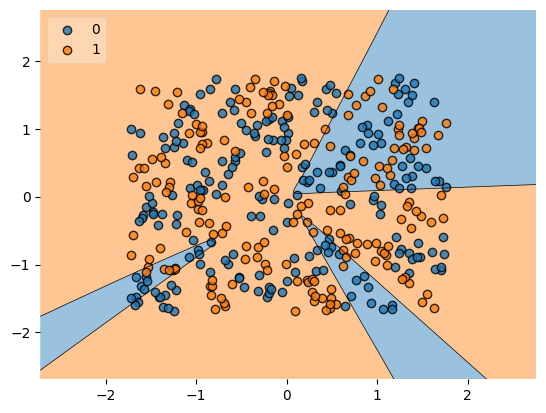
\includegraphics[width = 1in]{../images/regions/0-region-f.png}} &
\subfloat[10 epochs]{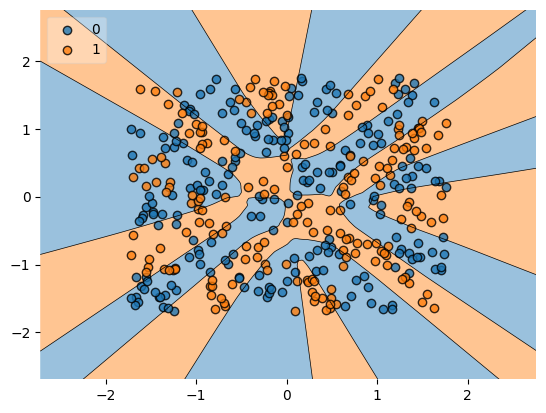
\includegraphics[width = 1in]{../images/regions/10-region-f.png}} &
\subfloat[20 epochs]{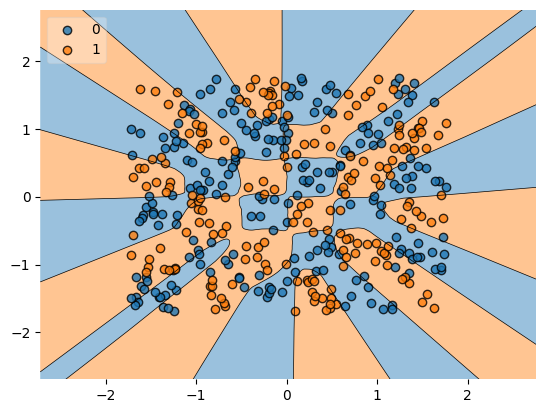
\includegraphics[width = 1in]{../images/regions/20-region-f.png}}\\
\subfloat[30 epochs]{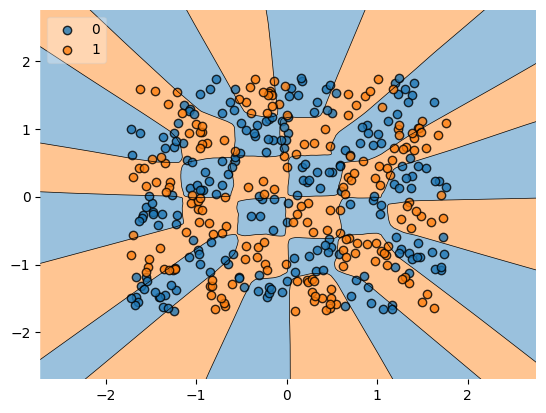
\includegraphics[width = 1in]{../images/regions/30-region-f.png}} &
\subfloat[40 epochs]{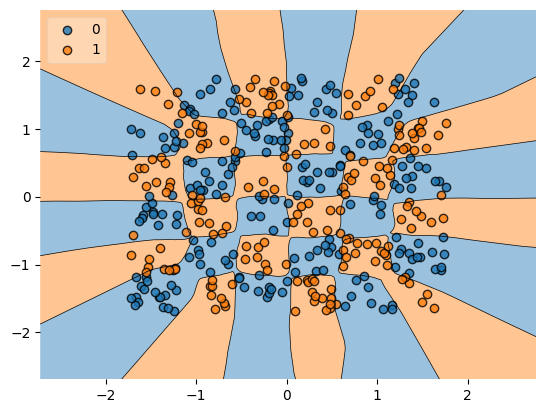
\includegraphics[width = 1in]{../images/regions/40-region-f.png}} &
\subfloat[50 epochs]{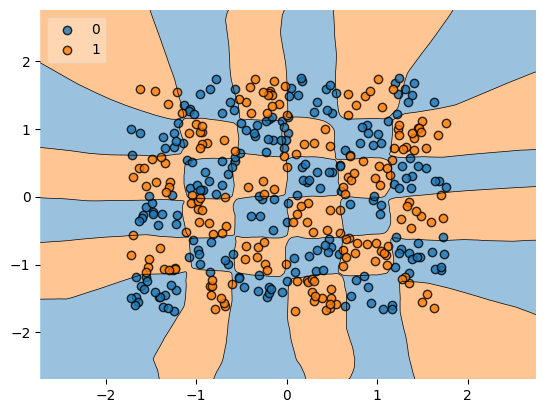
\includegraphics[width = 1in]{../images/regions/50-region-f.png}}\\
\subfloat[60 epochs]{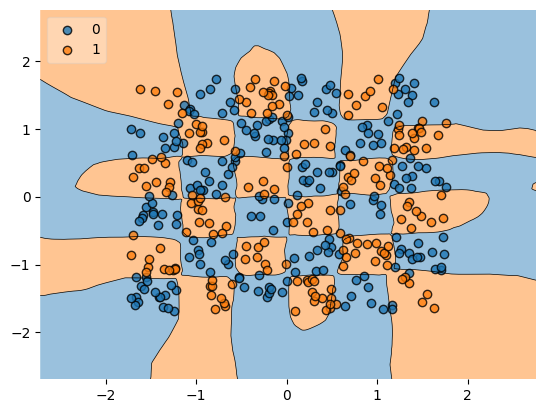
\includegraphics[width = 1in]{../images/regions/60-region-f.png}} &
\subfloat[70 epochs]{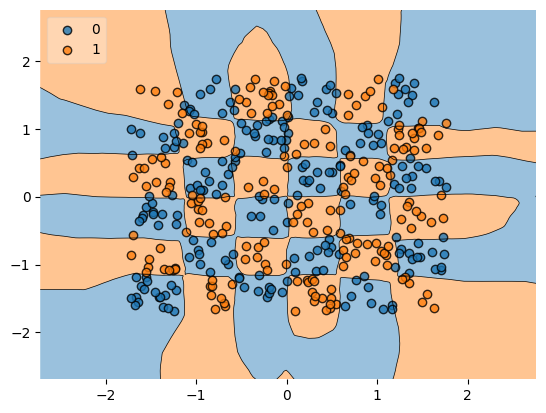
\includegraphics[width = 1in]{../images/regions/70-region-f.png}} &
\subfloat[80 epochs]{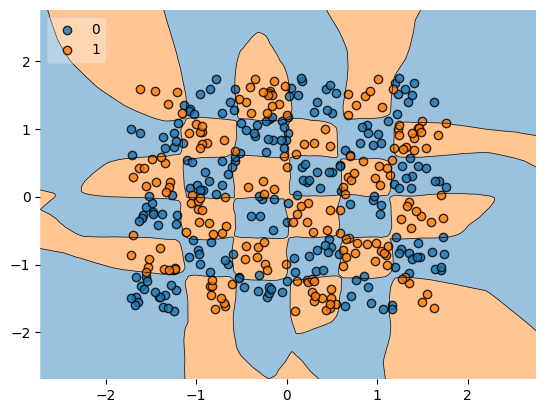
\includegraphics[width = 1in]{../images/regions/80-region-f.png}} 
\end{tabular}
\caption{Evolution of decision boundaries during the training}
\label{fig:decision}                                                                                                                                                           
\end{figure}

measure 
Figure \ref{fig:loss} and Figure \ref{fig:acc} plots the trend of the loss function and its accuracy over the validation set. The first one measures the absolute difference between the model's prediction and the actual value. \par
The second one represents the ratio between the number of correct predictions to the total number of predictions; it is preferable over the precision because accuracy treats
all classes with the same importance while precision measures the model's accuracy only in classifying a sample as positive.

\begin{figure}[ht!]
\centering                                                                        
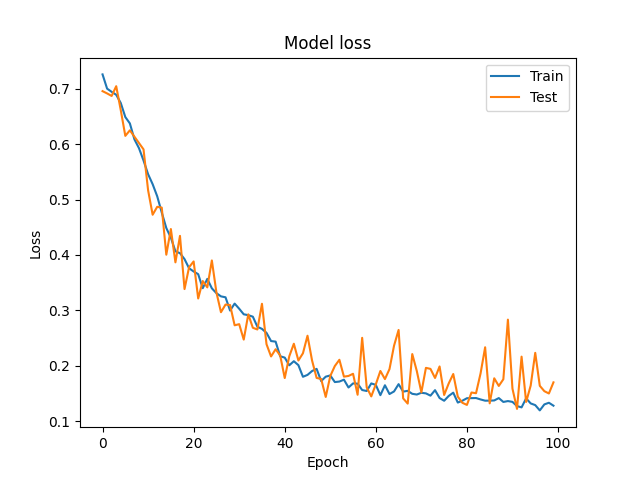
\includegraphics[width=3.5in]{../images/loss-4000-6-binary_crossentropy-adam-100-4.png}
\captionsetup{justification=centering}                                                                                                                                   
\caption{Loss}
\label{fig:loss}                                                                                                                                                           
\end{figure}


\begin{figure}[ht!]
\centering                                                                        
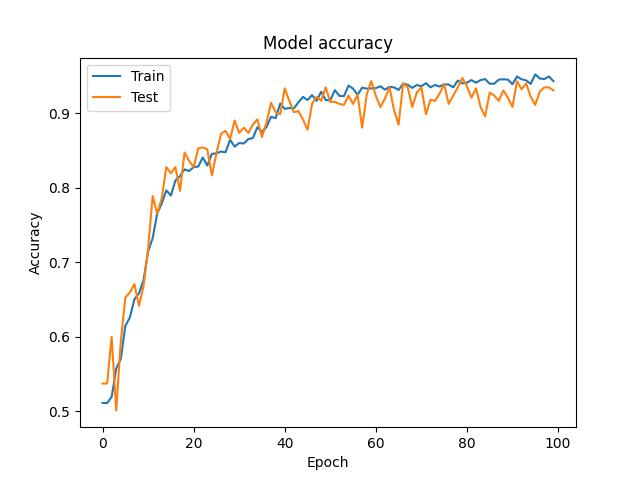
\includegraphics[width=3.5in]{../images/accuracy-4000-6-binary_crossentropy-adam-100-4.png}
\captionsetup{justification=centering}                                                                                                                                   
\caption{Accuracy}
\label{fig:acc}                                                                                                                                                           
\end{figure}



\section{Analysis}
From Figures \ref{fig:decision}, \ref{fig:loss} and \ref{fig:acc} we see that the model correctly classifies almost all the points after 60 epochs (accuracy $\geq 90\%$). This is a good result but we expected that the model could figure out what is the general rule under the provided classification.  
As we can see from Figure \ref{fig:decision}, as the accuracy of the model increases, it is clear that the model fails to recognize the \emph{check pattern} itself. Even if it is true that the accuracy reaches a score of $93\%$, the model overfits the data and could not generalize the pattern beyond the region occupied by training data. 
This means that a point outside the original training set (\emph{e.g.} $(9, 19)$) is classified by the model in the same way of the nearest checker (\emph{e.g.} orange instead of blue, even if the checker on its left is orange). \par
What happens is that the pattern predicted by the model is a checkerboard with the external checkers stretched infinitely outwards.
Figure \ref{fig:trend} shows a simplified trend in model's prediction if we increase the number of epochs.

\begin{figure}[ht!]
\centering                                                                        
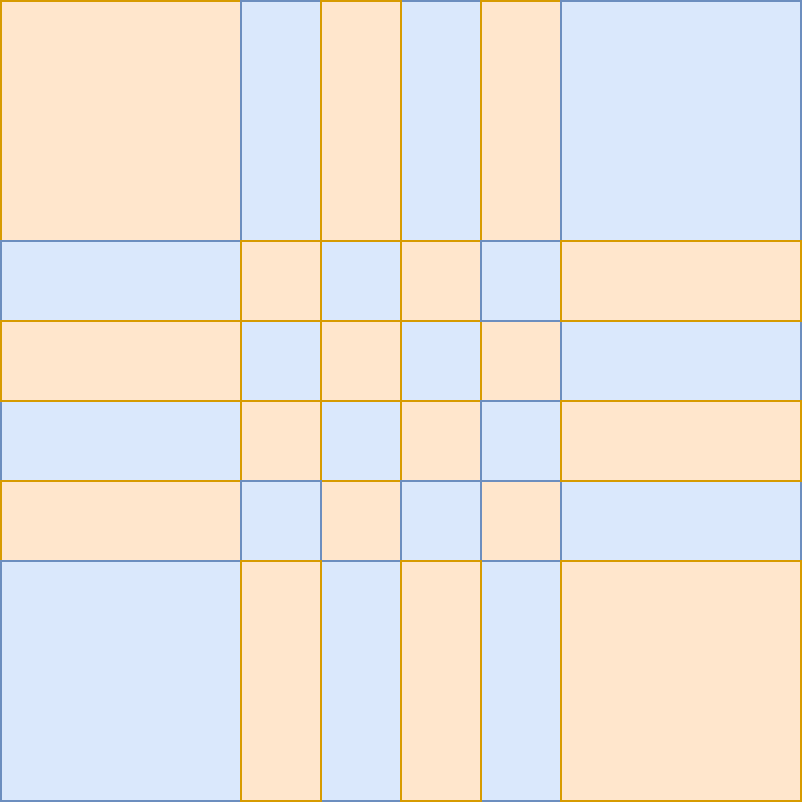
\includegraphics[width=2.5in]{../images/trend.png}
\captionsetup{justification=centering}                                                                                                                                   
\caption{Trend of the decision boundaries of the model}
\label{fig:trend}                                                                                                                                                           
\end{figure}

\section{Alternative problem}
The following problem is a variation of the previously presentend one. What is changing is the number of samples (from 4000 to 1000) and the number of checkers (from 36 to 400). This means that the frequency of samples is much more rare while leaving almost unchanged means and variation ($\mu=15.09$, $\sigma=8.64$). \par
Figure \ref{fig:checkerboard2} shows the new problem and it is impossible for the human brain to recognize the \emph{checker pattern}. The checkers are too thin and the data is not enough in order to recognize any pattern. \par
\begin{figure}[ht!]
\centering                                                                        
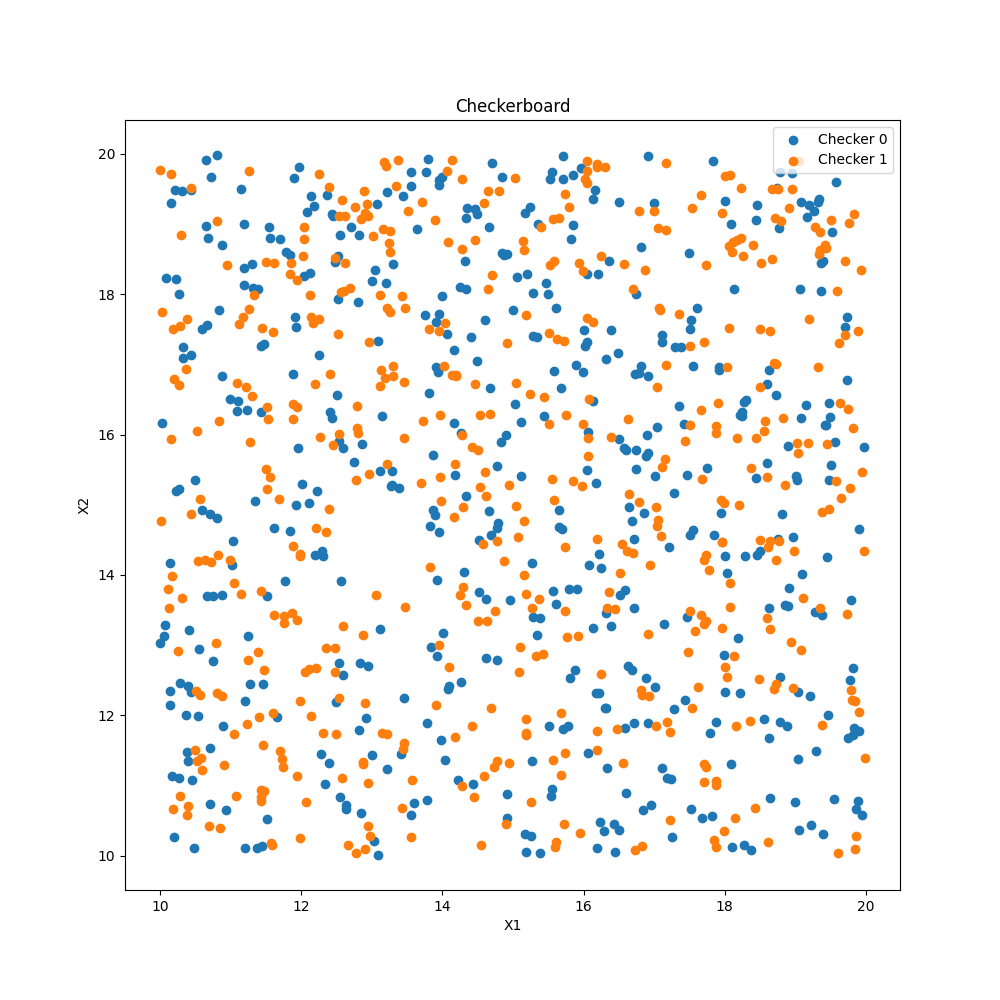
\includegraphics[width=3.5in]{../images/checkerboard-2.png}
\captionsetup{justification=centering}                                                                                                                                   
\caption{Visualization of the dataset of the alternative problem}
\label{fig:checkerboard2}                                                                                                                                                           
\end{figure}
The model, without any surprise, performs much worse: the maximum accuracy is $\sim55\%$, the loss remains quite high and it never converges (Figure \ref{fig:losacc})

\begin{figure}%
    \centering
    \subfloat[\centering Loss]{{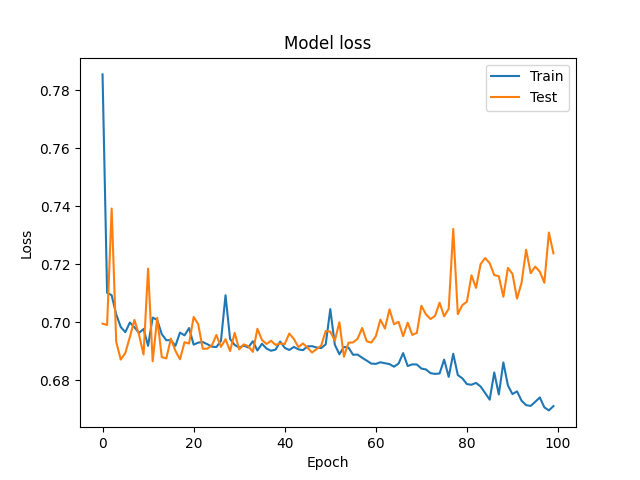
\includegraphics[width=5cm]{../images/loss-1000-20-binary_crossentropy-adam-100-4.png} }}%
    \qquad
    \subfloat[\centering Accuracy]{{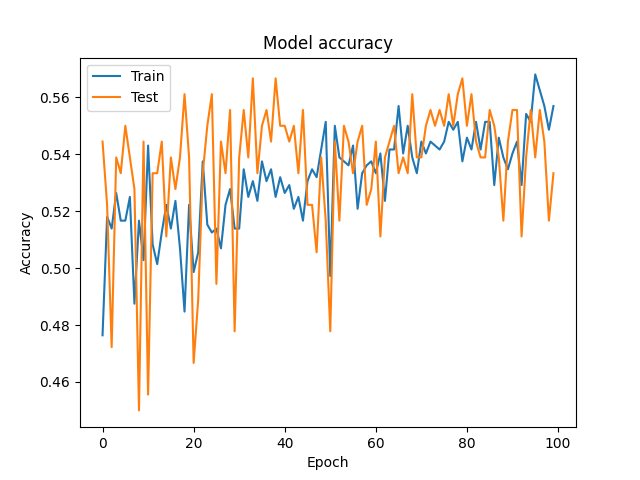
\includegraphics[width=5cm]{../images/accuracy-1000-20-binary_crossentropy-adam-100-4.png} }}%
    \caption{Loss and accuracy plots of the alternative problem}%
    \label{fig:losacc}%
\end{figure}

Figure \ref{fig:decision2} shows how the model could not find any pattern, changing quite frequently its decision boundaries

\begin{figure}[ht!]
\begin{tabular}{cccc}
\subfloat[1 epoch]{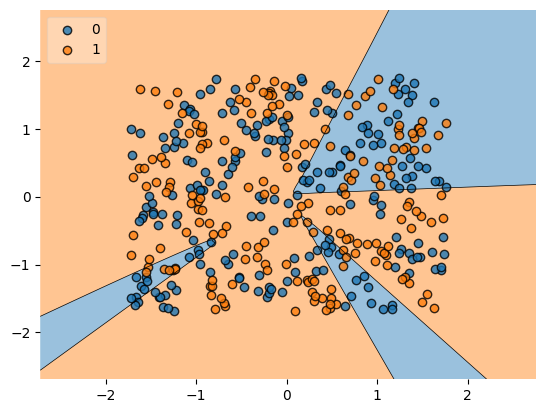
\includegraphics[width = 1in]{../images/regions/0-region.png}} &
\subfloat[10 epochs]{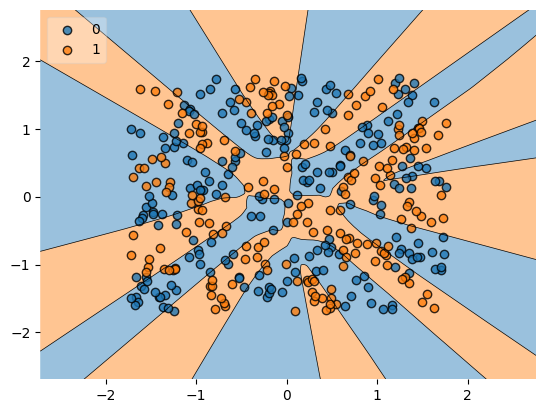
\includegraphics[width = 1in]{../images/regions/10-region.png}} &
\subfloat[20 epochs]{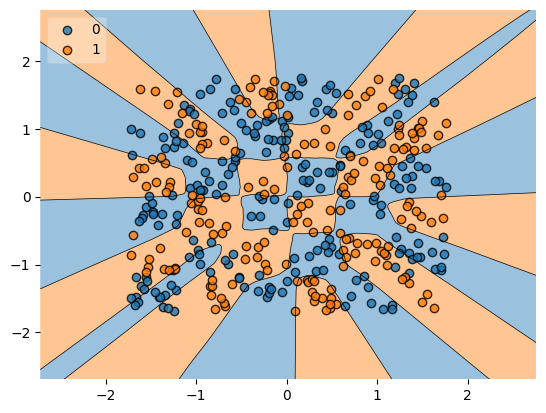
\includegraphics[width = 1in]{../images/regions/20-region.png}}\\
\subfloat[30 epochs]{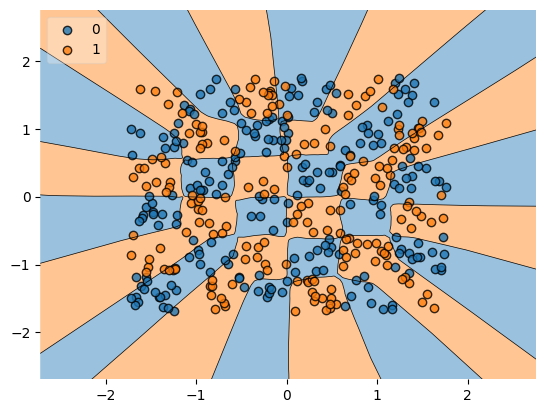
\includegraphics[width = 1in]{../images/regions/30-region.png}} &
\subfloat[40 epochs]{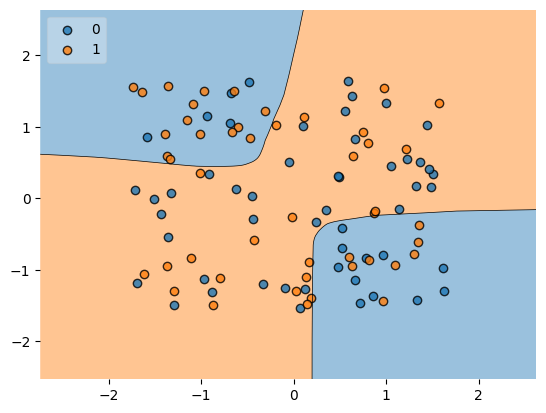
\includegraphics[width = 1in]{../images/regions/40-region.png}} &
\subfloat[50 epochs]{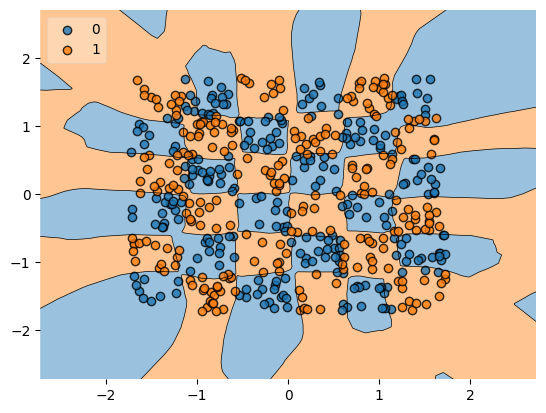
\includegraphics[width = 1in]{../images/regions/50-region.png}}\\
\subfloat[60 epochs]{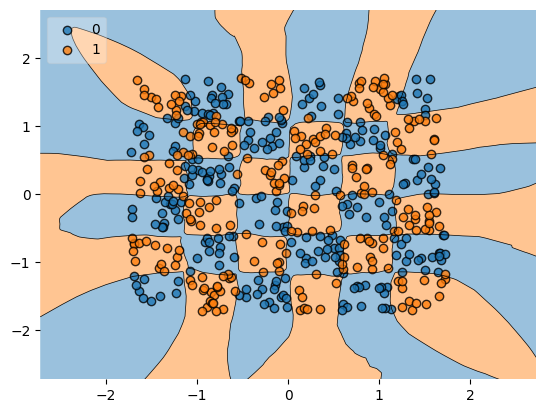
\includegraphics[width = 1in]{../images/regions/60-region.png}} &
\subfloat[70 epochs]{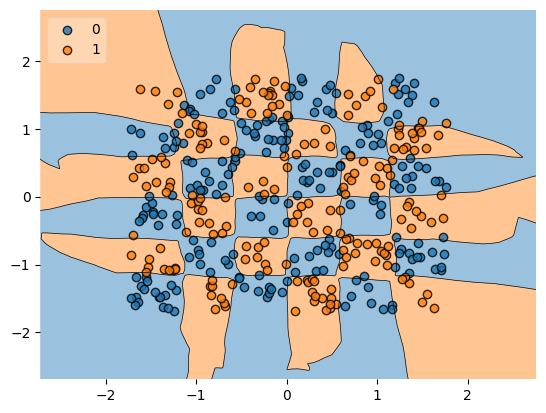
\includegraphics[width = 1in]{../images/regions/70-region.png}} &
\subfloat[80 epochs]{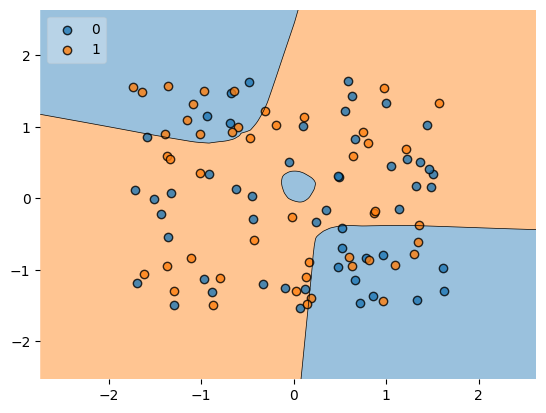
\includegraphics[width = 1in]{../images/regions/80-region.png}} 
\end{tabular}
\caption{Evolution of decision boundaries during the training of the alternative problem}
\label{fig:decision2}                                                                                                                                                           
\end{figure}


\section{Other experiments}
In this section we briefly documented the experiments with other optimizers: \emph{SGD} and \emph{RMSprop}. 
Even if their results where good, they converged slower than \emph{Adam}. \par

\emph{RMSprop} converges better than \emph{SGD} but it has difficulties on escaping local minima, having the loss function over test data to be more swinging (Figure \ref{fig:r1}).


\begin{figure}[ht!]
\centering                                                                        
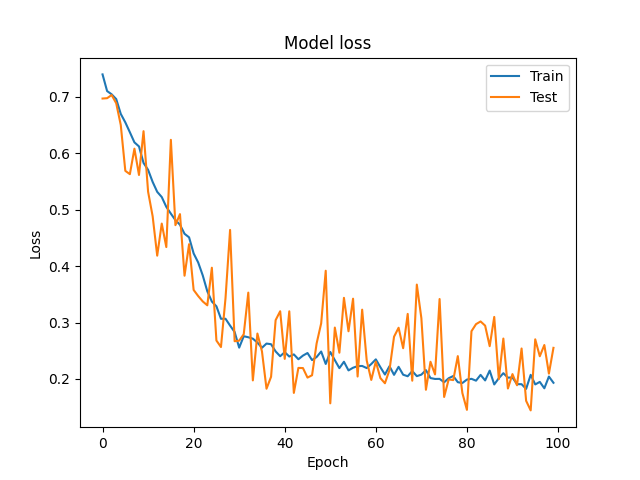
\includegraphics[width=3.5in]{../images/loss-4000-6-binary_crossentropy-rmsprop-100-4.png}
\captionsetup{justification=centering}                                                                                                                                   
\caption{Loss of \emph{RMSprop}}
\label{fig:r1}
\end{figure}

\begin{figure}[ht!]
\centering                                                                        
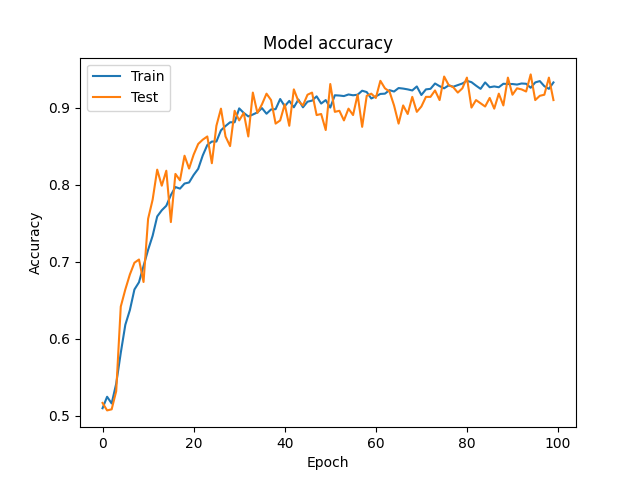
\includegraphics[width=3.5in]{../images/accuracy-4000-6-binary_crossentropy-rmsprop-100-4.png}
\captionsetup{justification=centering}                                                                                                                                   
\caption{Accuracy of \emph{RMSprop}}
\label{fig:r2}
\end{figure}


\emph{SGD} converges slower than \emph{RMSprop} but seems to be slighty better in escaping local minima (Figure \ref{fig:s1}).


\begin{figure}[ht!]
\centering                                                                        
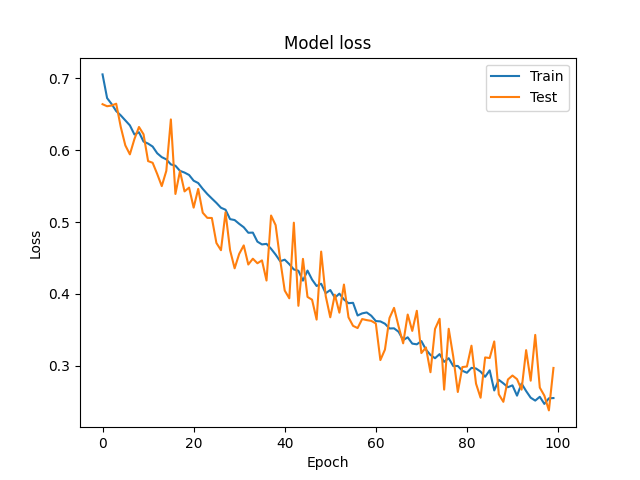
\includegraphics[width=3.5in]{../images/loss-4000-6-binary_crossentropy-sgd-100-4.png}
\captionsetup{justification=centering}                                                                                                                                   
\caption{Loss of \emph{SGD}}
\label{fig:s1}
\end{figure}

\begin{figure}[ht!]
\centering                                                                        
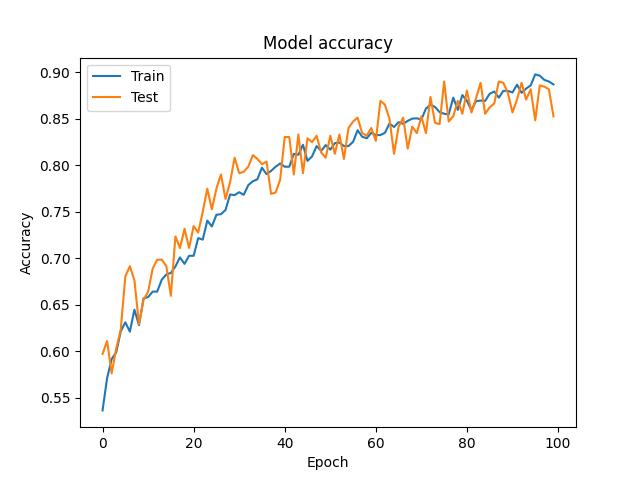
\includegraphics[width=3.5in]{../images/accuracy-4000-6-binary_crossentropy-sgd-100-4.png}
\captionsetup{justification=centering}                                                                                                                                   
\caption{Accuracy of \emph{SGD}}
\label{fig:s2}
\end{figure}




\bibliographystyle{ieeetr}
\bibliography{Bibliography}

\begin{thebibliography}{9}

\bibitem{nvidia} 
NVIDIA Developer: Turing tuning guide,
\\\texttt{\href{https://docs.nvidia.com/cuda/turing-tuning-guide/index.html}{https://docs.nvidia.com/cuda/turing-tuning-guide/index.html}}


\bibitem{fletcher} 
Fletcher, J. G. (January 1982). \textit{An Arithmetic Checksum for Serial Transmissions}. IEEE Transactions on Communications. COM-30 (1): 247–252. 
\href{https://ieeexplore.ieee.org/document/1095369}{doi:10.1109/tcom.1982.1095369}
\end{thebibliography}


\end{document}









